\section{Auswertung}
\label{sec:Auswertung}

\subsection{Überprüfung der Bragg Bedingung}

In Tabelle \ref{tab:braggbed} sind die Messwerte zur Überprüfung der braggschen
Bedingung dargestellt. Diese sind in Abbildung \ref{fig:braggbed} als Graph dargestellt.
Das Maximum der Kurve liegt bei dem Winkel
\begin{equation}
  \theta_\text{mess} = \SI{28.4}{\degree}.
\end{equation}

Der Sollwert für das Maximum lautet
\begin{equation}
  \theta_\text{soll} = \SI{28}{\degree}.
\end{equation}

\begin{figure}
  \centering
  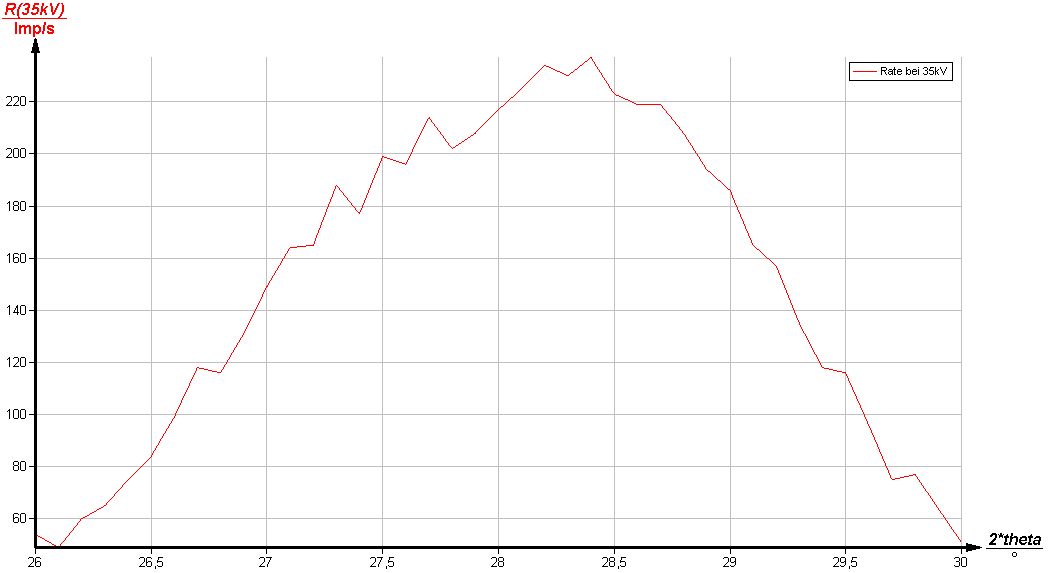
\includegraphics[height=7cm]{Daten/braggbedingung.png}
  \caption{Graph zur Überprüfung der Bragg Bedingung. Es sind die Impulse pro
  Sekunde gegen den Winkel aufgetragen.}
  \label{fig:braggbed}
\end{figure}

\begin{table}[h]
  \centering
  \begin{tabular}{S S}
    \toprule
    {$\theta/\si{\degree}$} & {$U\:/\:\si{\milli\volt}$}\\
    \midrule
    1 & 637.2\\
    \bottomrule
  \end{tabular}
  \caption{Messwerte zur Überprüfung der Bragg Bedingung.}
  \label{tab:braggbed}
\end{table}

\subsection{Das Emissionsspektrum einer CU-Röntgenröhre}

In Tabelle \ref{tab:emission} sind die Messwerte zur Bestimmung des
Emissionsspektrum einer CU-Röntgenröhre abgebildet. Der zugehörige Graph ist
ist in Abbildung \ref{fig:emission} dargestellt.

\begin{figure}
  \centering
  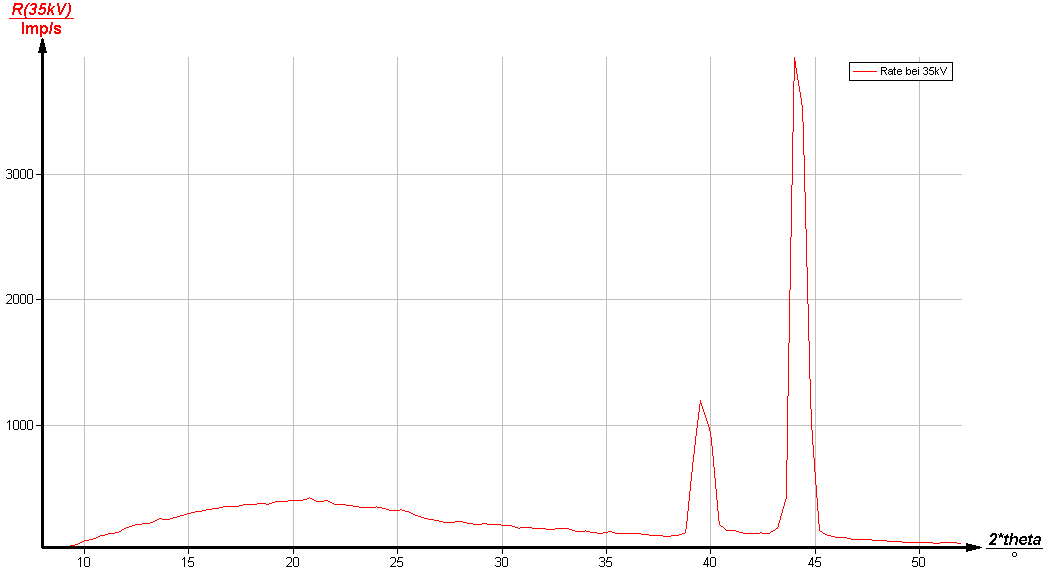
\includegraphics[height=7cm]{Daten/emissionsspektrum.png}
  \caption{Graph des Emissionsspektrums der CU-Röntgenröhre. Es sind die
  Impulse pro Sekunde gegen den Winkel aufgetragen.}
  \label{fig:emission}
\end{figure}

\begin{table}[h]
  \centering
  \begin{tabular}{S S}
    \toprule
    {$\theta/\si{\degree}$} & {$U\:/\:\si{\milli\volt}$}\\
    \midrule
    1 & 637.2\\
    \bottomrule
  \end{tabular}
  \caption{Messwerte zur Bestimmung des Emissionsspektrums.}
  \label{tab:emission}
\end{table}

8,8	26,0

\subsection{Absorptionsspektren verschiedener Stoffe und ich mag dich nicht}

\subsubsection{Germanium}

Die Messwerte der Germaniumprobe sind in Tabelle \ref{tab:germanium} abgebildet
und als Graph in der Abbildung \ref{fig:germanium} dargestellt.
Die gemessene K-Kante befindet sich bei
\begin{equation}
  \theta_\text{Ge} = 
\end{equation}

Tabelle für copy and paste:
\begin{table}[h]
  \centering
  \begin{tabular}{S S}
    \toprule
    {$k$} & {$U\:/\:\si{\milli\volt}$}\\
    \midrule
    1 & 637.2\\
    3 & 212.4\\
    5 & 127.4\\
    7 & 91.03\\
    9 & 70.8\\
    \bottomrule
  \end{tabular}
  \caption{Amplituden Rechteckspannung.}
  \label{tab:rechtampl}
\end{table}
